\documentclass[a4paper,12pt]{report}
%\usepackage[margin=2.5]{geometry}
\usepackage[T1]{fontenc} 
\usepackage[applemac]{inputenc} 
\usepackage[danish]{babel}  % dansih letters 
\usepackage[pdftex]{graphicx} 
\usepackage{fancyhdr} % hoved- og sidefod 
\usepackage{wrapfig}
\pagestyle{fancy}
\fancyhead[LO, CE]{SADP}
\fancyhead[RO, CE]{Twitter - Echo}
\fancyfoot[R]{\thepage}
\fancyfoot[C]{}
\fancyfoot[l]{Malik Lund, Lars Nilesen \& Christian Tidemand}
\begin{document}
\tableofcontents
\pagebreak
\section*{ECHO - Tweet the n3rdy way}
\addcontentsline{toc}{section}{Echo - Tweet the nerdy way}
Dette er en introduktions manual, til at bruge siden Echo, som skal bruges til at dele information om n�rd ting s� som nye programmeringsprog eller smart ting, som man har opdaget.  \\
\section*{Lad os komme igang}
\addcontentsline{toc}{section}{Lad os komme igang}
Dette er den f�rste del af Echo du ser.
\begin{figure}[h]
	\centering
		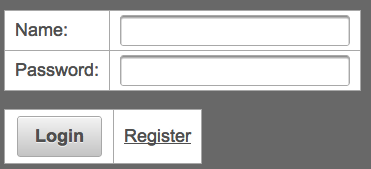
\includegraphics{image/login.png}
	\caption{Login siden}
\end{figure}
\subsection*{Hvis man har en bruger}
\addcontentsline{toc}{subsection}{Hvis man har en bruger}
Hvis man allerede har oprettet sig som bruger p� Echo, indtast en brugernavn i {\bf Name} feltet og adgangs koden indtastet i {\bf Password} feltet, her efter trykkes der {\bf Login} {\small (som ses i figur 1)}, hvor efter man bliver sendt vider til ens stream - se Stream.
\subsection*{Hvis man ikke har en bruger}
\addcontentsline{toc}{subsection}{Hvis man ikke har en bruger}
Hvis man ikke har f�et oprette en bruger skal man klikke p� {\bf Registre} hvorefter man bliver sendt vider til registerrings siden
\begin{figure}[h]
	\centering
		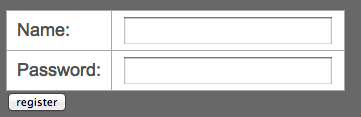
\includegraphics{image/register.png}
	\caption{Login siden}
\end{figure}
Her indtaster man sit �nskede brugernavn og kodeord og trykker registre. \\
Her kan ske to ting, ende bliver man bare godkendt og man kan derefter login. Hvis der derimod allerede er en bruger med det �nskede brugernavn, bliver man vider sendt til {\bf You fail} siden, hvor man her efter er n�d til at g� igennem processen igen.
\pagebreak
\section*{Stream}
\addcontentsline{toc}{section}{Stream}
\begin{figure}[h]
	\centering
		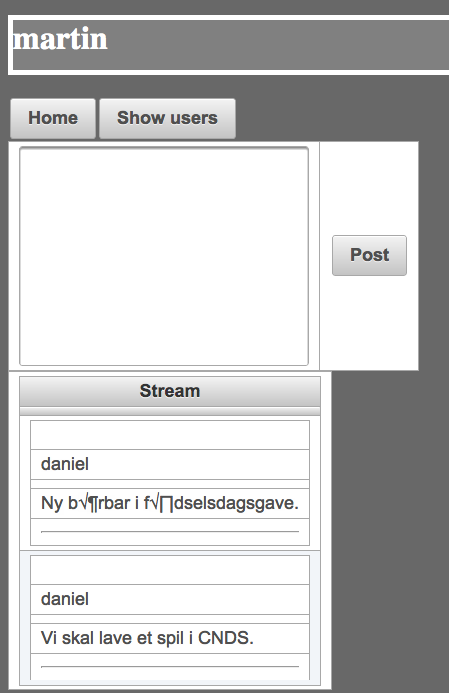
\includegraphics[width=70mm, height=90mm]{image/stream.png}
	\caption{Login siden}
\end{figure}
Ens Stream er hvor man f�r echos fra alle andre bruger som man f�lger, og hvor man kan se alle ens egne echos og sidst men ikke mindst f�r alle de echos som er specielt til en selv, ud over dette kan man f� adgang til at se alle bruger, og echo de ting man finder.
\end{document}